\documentclass{beamer}
\usepackage[utf8]{inputenc}
\usepackage[spanish]{babel}

\usepackage{latexsym,amsmath,xcolor,bm, amssymb, color, tikz, graphicx, amsthm, mathtools}
\usepackage{algorithm}
\usepackage{algorithmic}
\usepackage{hyperref}
\usepackage{float}     
\usepackage{CJKutf8}
\usepackage{multicol}

\graphicspath{{../logos/}{fotos/}}

\DeclareMathOperator*{\argmax}{arg\,max}
\DeclareMathOperator*{\argmin}{arg\,min}
\DeclareMathOperator{\sign}{sign}
\DeclareMathOperator{\Tr}{Tr}

\makeatletter
\DeclareRobustCommand\onedot{\futurelet\@let@token\@onedot}
\def\@onedot{\ifx\@let@token.\else.\null\fi\xspace}
\def\eg{\emph{e.g}\onedot} 
\def\Eg{\emph{E.g}\onedot}
\def\ie{\emph{i.e}\onedot} 
\def\Ie{\emph{I.e}\onedot}
\def\cf{\emph{c.f}\onedot} 
\def\Cf{\emph{C.f}\onedot}
\def\etc{\emph{etc}\onedot} 
\def\vs{\emph{vs}\onedot}
\def\wrt{w.r.t\onedot} 
\def\dof{d.o.f\onedot}
\def\etal{\emph{et al}\onedot}
\makeatother


\usetheme{Madrid}
\useinnertheme{circles}


\definecolor{ColorUNLP}{HTML}{8c0011} 
\usecolortheme[named=ColorUNLP]{structure}



%------------------------------------------------------------
% Info de la presentación
\title[Charla Panel: Pablo Heiber]{Charla Panel con Pablo Heiber}
\subtitle{De Competidor en ICPC World Finals a Organizador de Google Code Jam}

\author[Pablo Heiber]
{Invitado Especial: \textbf{Pablo Heiber} \\ \small Moderadores: Matías Ramos y Agustín Gutiérrez}

\institute[]{Universidad Nacional de La Plata – Facultad de Informática}
\date[TC 2026]{Training Camp Argentina 2026}
\titlegraphic{
\includegraphics[clip,height=2cm,keepaspectratio]{logoTC.pdf}}
%------------------------------------------------------------


%------------------------------------------------------------
% Indice automático al comenzar cada sección
\AtBeginSection[]
{
  \begin{frame}
    \frametitle{Estructura de la Charla}
    \tableofcontents[currentsection]
  \end{frame}
}
%------------------------------------------------------------


\begin{document}


% Diapositiva de Título
\frame{\titlepage}


% --- Organizadores y Sponsors ---
\begin{frame}{Gracias Sponsors!}
    \begin{columns}[t]
        \column{0.5\textwidth}
        \centering
        Organiza\\
        \vspace{0.5cm}
        
\includegraphics[width=0.6\textwidth,keepaspectratio]{logo_aapc.png}\\
        \vspace{0.3cm}
        
\includegraphics[width=0.8\textwidth,keepaspectratio]{unlp_informatica.png}
        \column{0.5\textwidth}
        \centering
        Diamond Sponsor\\
        \vspace{0.5cm}
        
\includegraphics[width=0.8\textwidth,keepaspectratio]{GTSlogo.jpeg}
    \end{columns}
\end{frame}


% Diapositiva de Contenido General
\begin{frame}{Estructura de la Charla}
    \tableofcontents
\end{frame}


% ============================================================
\section{Introducción}
% ============================================================

\begin{frame}{¿Quién es Pablo Heiber?}
    \begin{block}{Trayectoria Destacada}
        \begin{itemize}
            \item \textbf{Competidor Elite}: Dos veces finalista de la ICPC World Finals y finalista de la Google Code Jam.
            \item \textbf{Creador de Problem Statements}: Problemsetter para competencias regionales de ICPC y comités de problemas mundiales.
            \item \textbf{Ingeniero en Google}: Software Engineer y organizador de la Google Code Jam hasta su histórica edición de 2023.
            \item \textbf{Formación Académica}: Licenciado y Doctor en Ciencias de la Computación de la Universidad de Buenos Aires (UBA).
        \end{itemize}
    \end{block}
\end{frame}


% ============================================================
\section{Etapa como Competidor}
% ============================================================

\begin{frame}{World Finals 2005 (Shanghái)}
    \begin{columns}
        \column{0.55\textwidth}
        \begin{block}{El Camino a Shanghái}
            \begin{itemize}
                \item Representó a la \textbf{Universidad de Buenos Aires (UBA)}.
                \item Equipo integrado junto a \textbf{Hernán Bandura} y \textbf{Francisco Roslan}.
                \item Ese mismo año 2005 también se clasificó y compitió como \textbf{finalista mundial en la Google Code Jam}.
            \end{itemize}
        \end{block}
        
        \column{0.45\textwidth}
        \centering
        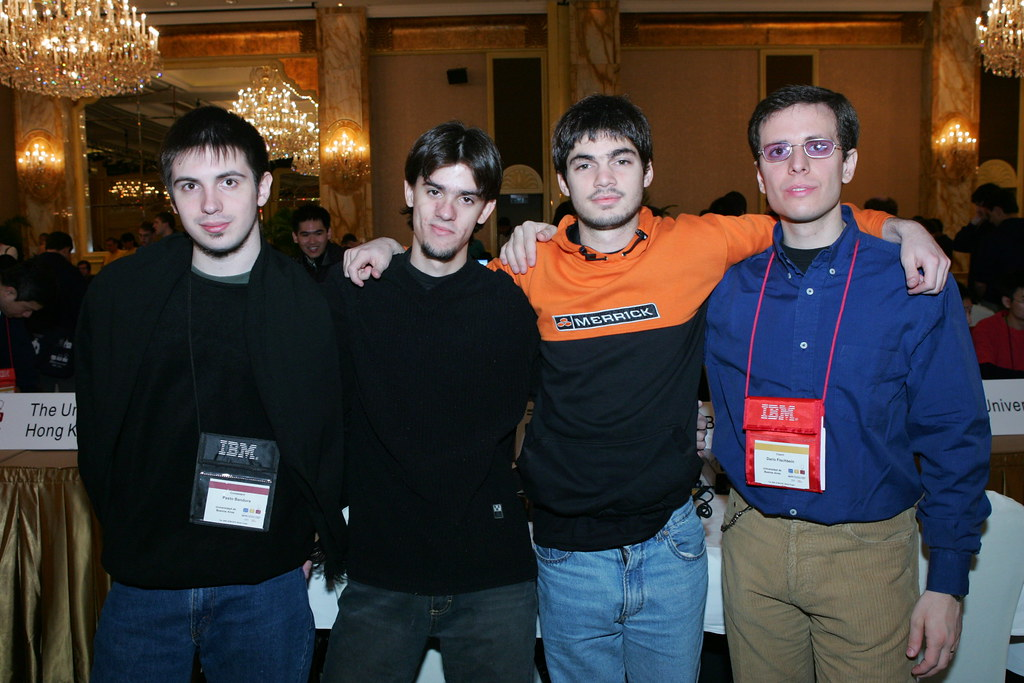
\includegraphics[width=1.0\textwidth,keepaspectratio]{wf2005.jpg}
        \\ \vspace{0.1cm}
        \tiny{Pablo Heiber en la ICPC World Finals 2005 en Shanghái, China.}
    \end{columns}
\end{frame}


\begin{frame}{World Finals 2007 (Tokio)}
    \begin{columns}
        \column{0.55\textwidth}
        \begin{block}{Consagración en Latinoamérica}
            \begin{itemize}
                \item Compitió representando a la \textbf{Universidad de Buenos Aires (UBA)}.
                \item Equipo integrado por \textbf{Pablo Heiber}, \textbf{Alejandro Deymonnaz} y \textbf{Francisco Roslan}.
                \item \textbf{Latin American Champions}!
                \item Alcanzó la posición \textbf{14 del mundo}.
                \item Quedaron a tan solo \textbf{un problema} de obtener una medalla de bronce.
            \end{itemize}
        \end{block}
        
        \column{0.45\textwidth}
        \centering
        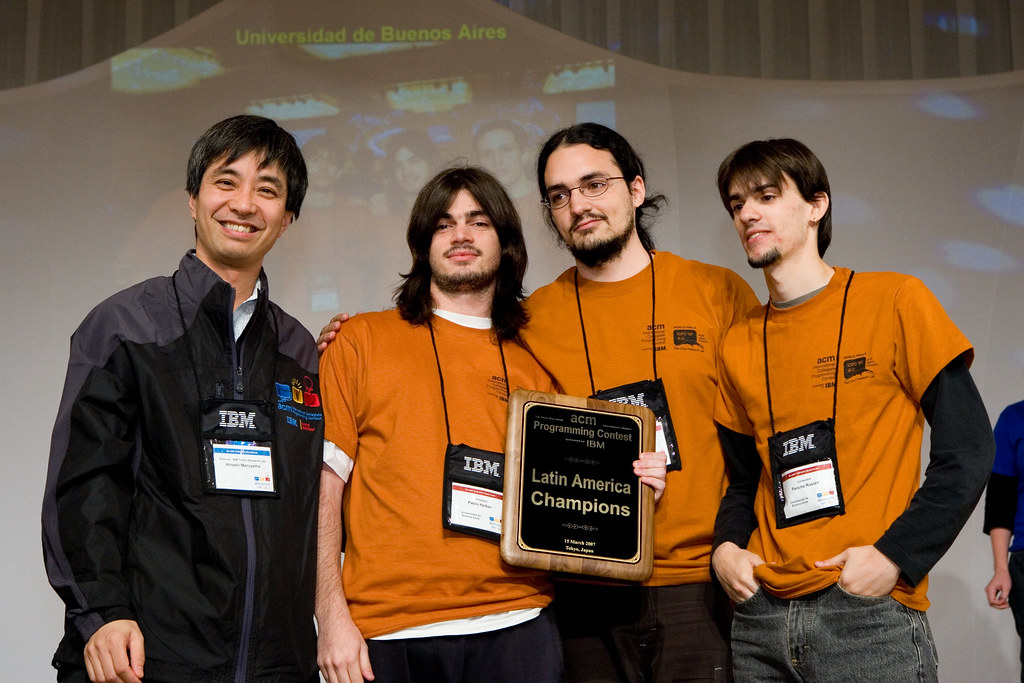
\includegraphics[width=1.0\textwidth,keepaspectratio]{wf2007.jpg}
        \\ \vspace{0.1cm}
        \tiny{Recibiendo el premio de Campeones Latinoamericanos en Tokio, Japón (2007).}
    \end{columns}
\end{frame}


% ============================================================
\section{Problemsetter y Juez}
% ============================================================

\begin{frame}{Problemsetter en ICPC Latam (2011-2015)}
    \begin{columns}
        \column{0.45\textwidth}
        \begin{block}{Creando Problem Statements}
            \begin{itemize}
                \item Miembro del comité de problemas de ICPC Latam.
                \item Diseñador de problem statements en la región.
                \item Aporte a la rigurosidad y calidad del entrenamiento regional.
            \end{itemize}
        \end{block}
        
        \column{0.26\textwidth}
        \centering
        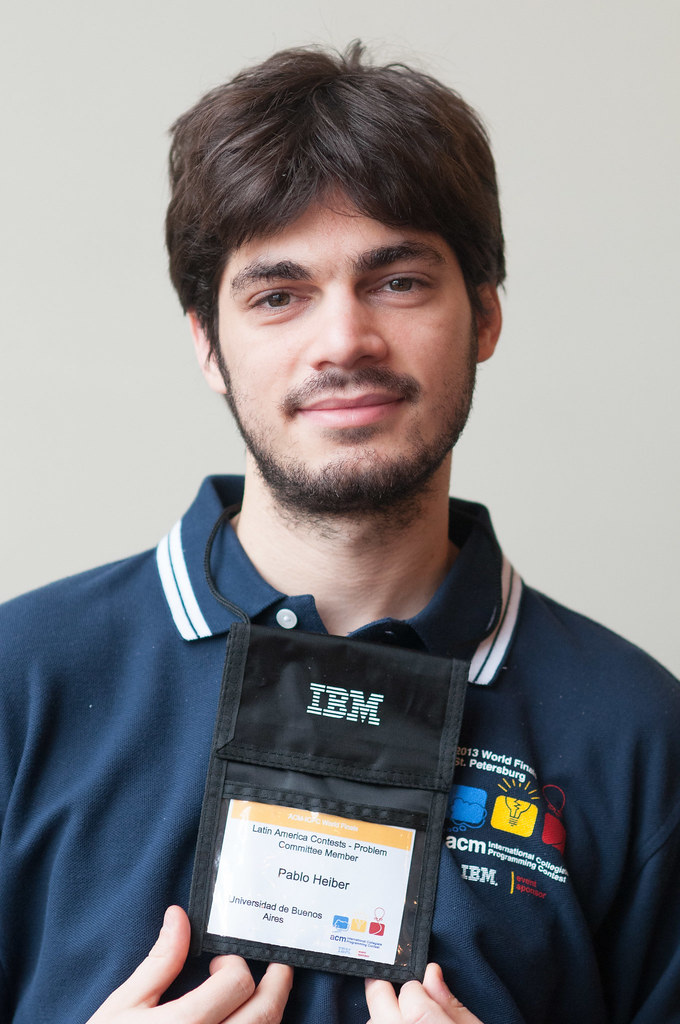
\includegraphics[width=1.0\textwidth,keepaspectratio]{setter1.jpg}
        
        \column{0.26\textwidth}
        \centering
        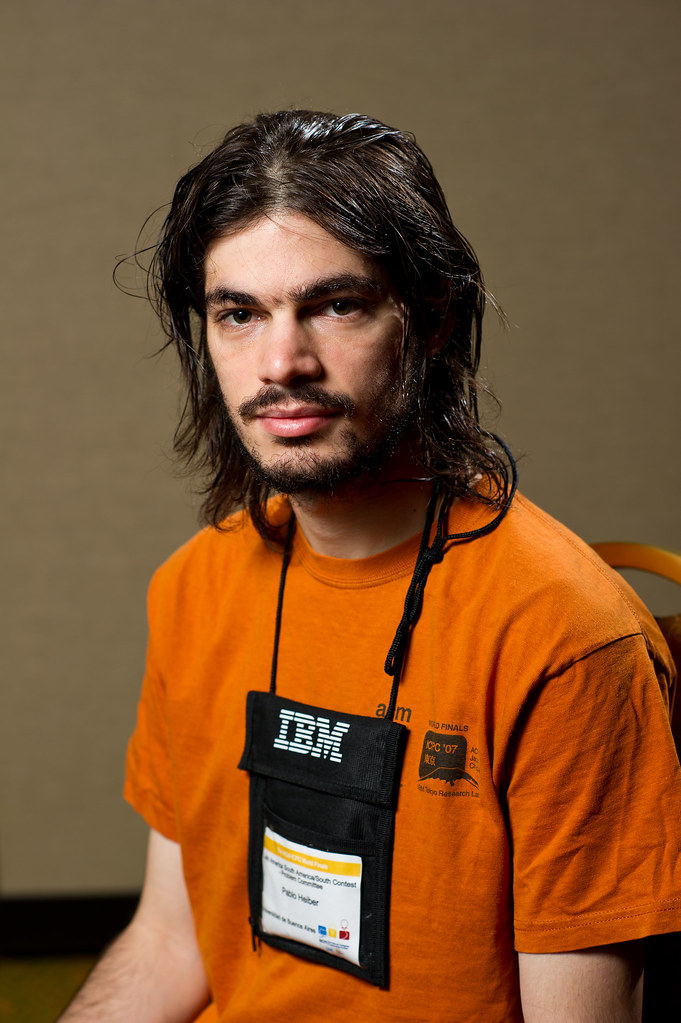
\includegraphics[width=1.0\textwidth,keepaspectratio]{setter2.jpg}
    \end{columns}
    \vspace{0.2cm}
    \centering
    \tiny{Pablo Heiber trabajando en el jurado de la ICPC Latam.}
\end{frame}


% ============================================================
\section{Organización de Google Code Jam}
% ============================================================

\begin{frame}{Google Code Jam (Hasta 2023)}
    \begin{columns}
        \column{0.55\textwidth}
        \begin{block}{Organización del Certamen}
            \begin{itemize}
                \item Lideró el diseño de problem statements e infraestructura como Ingeniero de Software.
                \item Desarrolló y mantuvo la plataforma y el \textbf{juez online} utilizado para las competencias.
                \item Responsable de la calidad de los problem statements resueltos por cientos de miles de competidores mundialmente.
                \item Organizó y acompañó el torneo hasta su histórica edición de cierre en \textbf{2023}.
            \end{itemize}
        \end{block}
        
        \column{0.45\textwidth}
        \centering
        
\includegraphics[width=0.8\textwidth,height=1.5cm,keepaspectratio]{gcj_logo.png}
        \\ \vspace{0.2cm}
        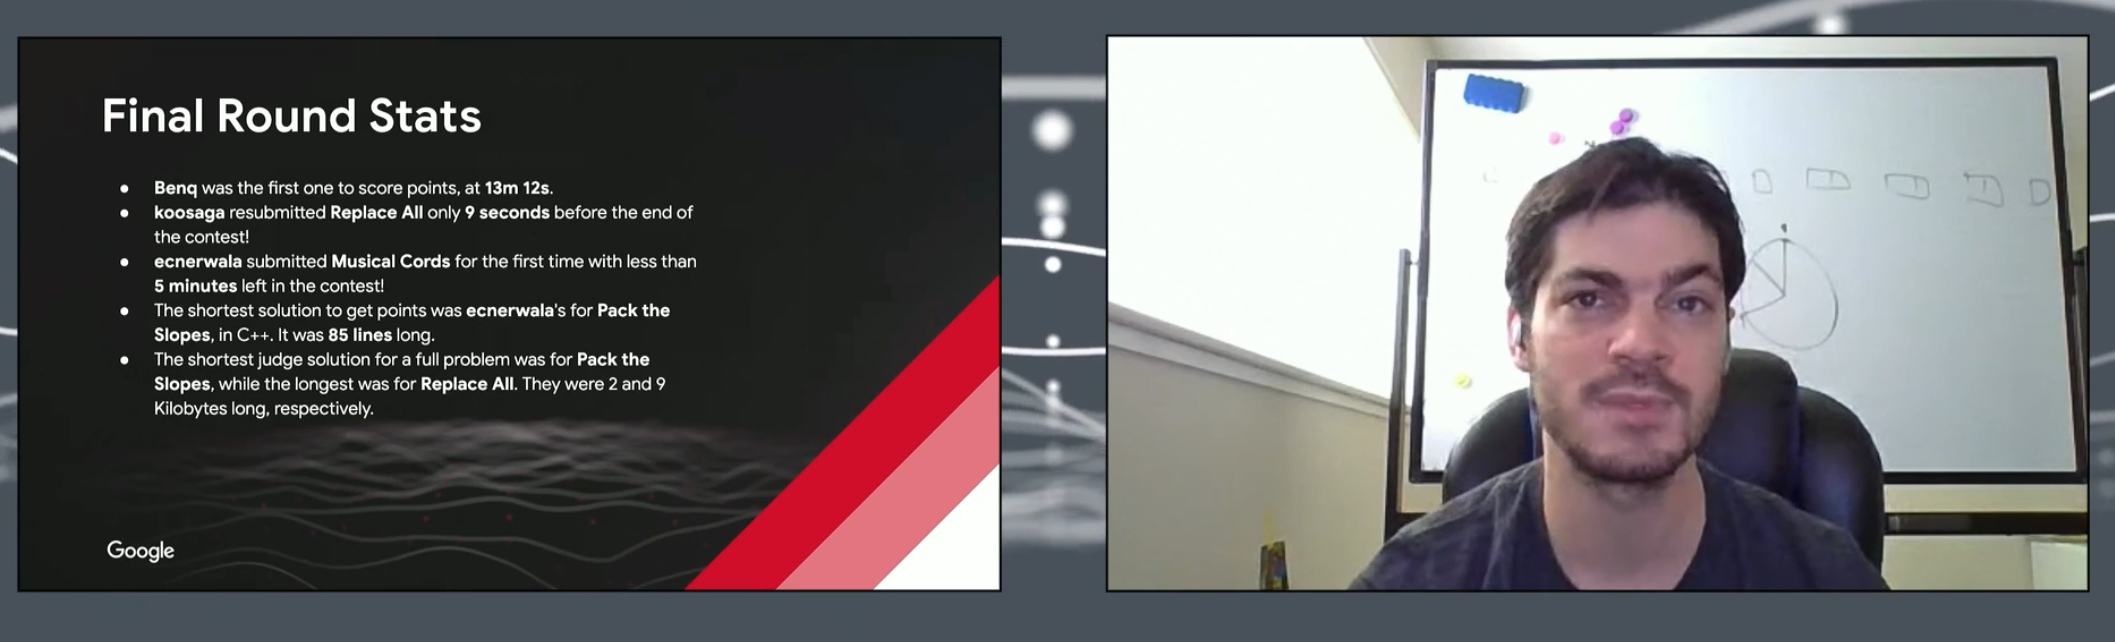
\includegraphics[width=1.0\textwidth,height=3cm,keepaspectratio]{gcj_pablo.png}
        \\ \vspace{0.1cm}
        \tiny{Pablo Heiber en la transmisión de la Final de GCJ 2020.}
    \end{columns}
\end{frame}


% ============================================================
\section{Panel de Debate y Preguntas}
% ============================================================

\begin{frame}{Preguntas y Debate}
    \begin{alertblock}{Espacio Abierto}
        ¡Aprovechemos la presencia de Pablo Heiber para conversar sobre:
        \begin{itemize}
            \item Consejos para preparar competencias nacionales e internacionales.
            \item Cómo crear problemas interesantes y balanceados.
            \item Anécdotas de las World Finals y Google Code Jam.
        \end{itemize}
    \end{alertblock}
\end{frame}


\begin{frame}{}
    \centering
    \Huge\color{ColorUNLP}{\textbf{¡Muchas gracias, Pablo!}}
    
    \vspace{1.2cm}
    \large
    Por tu tiempo, tus valiosos consejos y tu enorme aporte a la comunidad de programación competitiva.
    
    \vspace{1.0cm}
    \small
    Training Camp Argentina 2026
\end{frame}


\end{document}
